\section{GPU implementation of EmbedSOM}\label{sec:impl}

While EmbedSOM is relatively straightforward to parallelize for mainstream CPU architectures, several challenges appear when designing of an optimal implementation for contemporary GPUs.
In this section, we outline the key optimizations that allowed us to run the high-performance dimensionality reduction in EmbedSOM, and give an overview of the relative performance gains achieved by the algorithm choice.

Technically, the algorithm consists of two main parts that provide distinct implementation challenges:

\begin{itemize}
\item {\bfseries $k$-NN step}\quad
The search of $k$-nearest landmarks in $L$ for each data point from $X$ requires a highly irregular selection of indices of $k$ lowest values from columns of the dynamically computed distance matrix $L^T\cdot X$.

\item {\bfseries Projection step}\quad
Computation of the small linear system that is used to find the minimal-error-projection of a point, namely of projections $D_{uv}$ and the derivatives $\frac{\delta d_{uv}}{\delta x_i}$ (Section~\ref{sec:methods}), is difficult to optimize due to irregular memory access patterns of collecting the data for the computation.
\end{itemize}

% We carried out the implementation in NVIDIA CUDA~\cite{guide2013cuda}, the performance validation presented in the next sections is accordingly carried out only on NVIDIA hardware that supports CUDA.
% Despite our benchmarks being NVIDIA-specific, the presented kernels do not depend on any NVIDIA-specific functionality, and the results should be portable to other GPU programming frameworks (such as Vulkan Compute shaders) and hardware of other vendors.
% We expect that only minor adjustments will be required to compensate for GPU design differences, such as the 64-thread wavefronts on AMD devices.

In the following two sections, we describe in detail the optimizations of the CUDA implementation.

\subsection{$k$-NN selection step}\label{sec:impl-knn}

The task of the first part of the algorithm is to find $k$ nearest landmarks (from $L$) for every data point in $X$.
This comprises two sub-steps: computing Euclidean distances for every pair from $L$ and $X$ and performing point-wise reduction that selects a set of $k$ nearest landmarks for each of the $n$ points, based on the computed distances.

While the Euclidean distance computation is mathematically simple and embarrassingly parallel, achieving optimal throughput on GPUs is quite challenging~\cite{krulivs2017employing}.
In particular, the ratio between the data transfers and the arithmetic operations performed by each GPU core is heavily biased towards data transfers.
The overhead of data transfers is best prevented by finding a good caching pattern for the input data that is able to optimally utilize all hardware caches (L1 and L2), shared memory, and core registers.

The parallel implementation of the $k$-nearest neighbors search is even more challenging.
The $k$-NN problem is computed individually for each data point, which provides the space for possible parallelization.
However, concurrently processed instances of a na\"{i}ve $k$-NN implementation exhibit severe code divergence because the selection process is purely data-driven, and requires a high amount of memory allocated per core.
Optimally, the $k$-NN selection is realized by customized versions of parallel sorting algorithms, which are well-researched and possess existing GPU implementations~\cite{singh2018survey}.

Our implementation chooses to optimize both sub-steps since the ratio of the amount of required computations can be easily biased by the configuration of parameters $d$ and $k$.
In particular, processing high-dimensional datasets with a low $k$ parameter spends significantly more time in the distance computation, but lower-dimensional datasets with higher $k$ require more time in the nearest neighbor selection.

Concerning the perspective of software design, the implementation may use separate kernels for both sub-tasks or a single fused kernel.
Kernel separation provides better code modularity and much flexibility in work-to-thread division and data caching strategy, at the cost of having to materialize all the computed distances in the GPU global memory, thus significantly increasing the total amount of data transfers.
Contrary to that, a fused kernel may immediately utilize the computed distances in $k$-NN computation without transferring the data to global memory and interleaving the distance computations with $k$-NN may help to improve the ratio between computations and data transfers.
Since our initial observations showed that the overhead of the data transfers required for kernel communication is relatively high, we decided to implement only the fused variant for the sake of simplicity.
The usage of separate kernels might be interesting in the future, especially for extreme values of $d$ that diminish the relative cost of the distance data transfer.

\subsubsection{Available algorithms for $k$-NN}

There are many approaches to $k$-NN selection, varying in complexity and parameter-dependent performance. We implemented several of the possibilities (as described in this section) to substantiate our choice of the algorithm for GPU EmbedSOM.

As a baseline (labeled \Alg{Base}), we used the most straightforward approach to GPU parallelization which simply invokes original sequential code for every data point concurrently.
The \alg{Base} kernel is spawned in $n$ threads (one for each data point), and each thread computes the distance between its data point and all landmarks while maintaining an ordered array of $k$ nearest neighbors.
The array is updated by an insert-sort step performed for every new computed distance --- i.e., by starting at the end of the array and moving the new distance-index pair towards smaller values until it reaches the correct position.

\Alg{Shared} algorithm is a modified version of the baseline algorithm that utilizes shared memory as a cache, following the recommended optimization practice of improving performance by caching data that are reused multiple times~\cite{guide2013cuda}.
In this case, we cache the landmark coordinates, which are sufficiently small to fit in the shared memory for all tested parametrizations.

In \Alg{GridInsert} algorithm, we utilize the shared memory to cache both landmarks and points.
However, the limited size of shared memory imposes limitations of the amount of cached data. Hence, the algorithm was parametrized by the block height $h$ (number of cached points from $X$) and the block width $w$ (number of cached landmarks from $L$).
The algorithm runs in epochs, each of which first caches $h$ points and $w$ landmarks, and then computes $h \cdot w$ distance values using only data in shared memory.
While the distances are computed concurrently by the whole thread block, we chose to avoid explicit synchronization in the $k$-NN step, using only $h$ threads to incorporate the newly computed distances into $h$ separate $k$-NN results using the insert-sort steps.
The \alg{GridInsert} should achieve better throughput in the distance computation thanks to the caching, at the cost of slightly sub-optimal $k$-NN reduction; thus, giving the best performance on high-dimensional datasets and low values of $k$.

% The above algorithms focus solely on optimizing the distance computation; we further detail the possible optimizations of the $k$-NN selection.

% A straightforward way for computing the $k$ nearest neighbors in parallel is to sort an entire array of distances using a parallel sorting algorithm, then taking the first $k$ items.
% Although the overhead of storing the distances might be excessive, we expected the strategy to be competitive especially for large values of $k$ (approaching the total number of landmarks in the grid).
% We use this approach in \Alg{Radix} algorithm, which employs the highly-optimized sorting algorithm from the state-of-art CUB library~\cite{cub}.
% The algorithm allocates an entire thread block to process one input data point.
% The block cooperates on computing the Euclidean distances by dividing the landmarks evenly among the threads.
% The distances are stored along with indices in the shared memory block, which is then sorted by the CUB radix sort, and subsequently the first $k$ items are copied to the result buffer in global memory.
% Importantly, the whole block of $g$ distance-index pairs must fit in the shared memory, which imposes a limitation on the maximal amount of landmarks, and prevents much of the input caching in the shared memory, impacting the efficiency of distance computation.

Finally, improvising on our previous work~\cite{krulivs2015optimizing}, we implemented \Alg{Bitonic} $k$-NN selection algorithm, which utilizes routines from the highly parallelizable bitonic sorting algorithm.
Bitonic sorting is very suitable for parallel lockstep execution~\cite{krulivs2017employing}, and the capability to merge sorted sequences has allowed us to keep only $2k$ distances (instead of $g$) in the shared memory.
This method benchmarked the best on the average, so it is selected as default for EmbedSOM and we describe it more thoroughly in the following.


\subsubsection{Bitonic approach to $k$-NN}

The \alg{Bitonic} approach can be seen as a combination of the benefits of the other algorithms: It does not require materializing all distances in the memory to do a full sort and even though it does not use an elaborate input caching strategy like \alg{GridInsert}, it still gives interesting results because the data loading operations can be partially overlapped with bitonic sorting operations if enough warps are allocated to one streaming multiprocessor.

\begin{figure}
	\centering
	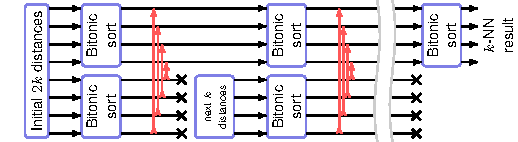
\includegraphics{embedsom/pic/bitonic.pdf}
	\caption{\alg{Bitonic} algorithm for $k$-NN selection ($k=4$). Each horizontal line represents a data item in the shared memory. Red lines represent comparators ensuring, that the intermediate $k$ `best' neighbors and in the top buffer.}
	\label{fig:bitonic-schema}
\end{figure}

The bitonic comparator network provides a building block that, given two buffers of size $k$ of neighbor distances sorted by bitonic sort, selects the closest $k$ of the neighbors in a single (parallel) operation, allowing us to quickly discard neighbors that do not belong into the $k$-neighborhood.
Applying this operation iteratively on $k$-sized blocks of distances sorted by the bitonic sort (as shown in Figure~\ref{fig:bitonic-schema}), we obtain a highly performing scheme that requires only $2k$ items present in the shared memory.
In particular, the shared memory always contains a $k$-block of distances (and corresponding indexes) that holds $k$ so-far-nearest neighbors, and one block of $k$ distances that are computed from $L$; in each iteration, both blocks are sorted by the bitonic sorter in parallel and merged by the bitonic comparator to move the distances of new nearest $k$ neighbors into the intermediate block.
The other block is then re-filled by a new set of $k$ distances from $L$.

Technically, each step of the sorting net requires $\frac{k}{2}$ comparators, thus optimally $\frac{k}{2}$ threads that work concurrently on the $h$-sized block.
Hence, we allocate $k$ threads for each data point, which alternate their work between computing a block of $k$ distances and performing two bitonic sorts on two $k$-sized blocks in parallel.
For simplicity, our implementation assumes that $k$ is always a power of $2$, and excessive output of the sorter is discarded.



\subsection{Projection step}\label{sec:impl-projection}

The second part of the dimensionality reduction method is the actual projection into the low-dimensional space.
The computation of the low-dimensional point position $x_i$ by EmbedSOM involves: 
(1) Conversion of the distances collected in the $k$-NN to scores;
(2) Orthogonal projection of $X_i$ to $k \choose 2$ lines generated by the $k$ neighbors to create contributions to the final approximation matrix;
(3) Solution of the resulting small linear system using Cramer's rule.

Since the first and the last steps are embarrassingly parallel problems with straightforward optimal implementation and since the second step is the most time demanding (performing $\mathcal{O}(k^2)$ operations on vectors of size $d$), we focus mainly on the orthogonal projections. Its computation is complicated by a highly irregular pattern of repeated accesses to an arbitrary $k$-size subset of $L$. We designed several algorithms that successively optimize the access patterns, detailed below.

The baseline algorithm \Alg{Base} uses the most straightforward parallel approach (similar to \alg{Base} $k$-NN), where each thread computes the projection of one single point sequentially so the concurrency is achieved only by processing multiple points simultaneously.
All data are stored in the global memory, and no explicit cache control is performed.

The irregular repeated access to the elements of $L$ hinders the performance of the baseline algorithm.
In the \Alg{Shared} algorithm, we chose to reorganize the workload so that each projection is computed by a whole block of threads that cooperatively iterate over the landmark pairs.
As a result, the input data of the orthogonal projection (i.e., the $k$ nearest neighbors from $L$ together with the distances, scores, and 2D versions of the landmarks) can be cached in shared memory.
The intermediate sub-results represented by $2\times3$ matrices are successively added into privatized copies of each thread to avoid explicit synchronization and aggregated at the end using a standard parallel reduction, enhanced with warp-shuffle instructions (a similar scheme is used in optimal CUDA k-means implementation~\cite{krulis2020detailed}).

Because the data transfers comprise a considerable portion of the \alg{Shared} algorithm execution time, we have optimized the transfers using alignment and data packing techniques, yielding the \Alg{Aligned} algorithm.
The implementation is based on using vector data types (e.g. \texttt{float4} in CUDA) to enable utilization of $128$-bit load/store instructions, which improves overall data throughput.
The vectorization comes only at a relatively small cost of aligning and padding the vectors to $16$-byte blocks.

\begin{figure}
\centering
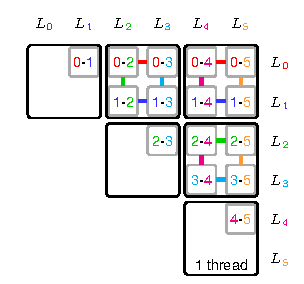
\includegraphics{embedsom/pic/reg-caching.pdf}
\caption{Detail of the caching of landmark data in \alg{Registers} projection kernel. Multiple landmark pairs (small boxes) are processed by each thread (large boxes). Caching of the landmark data in registers allows the reuse of loaded data (color lines), thus reducing the amount of memory accesses.}
\label{fig:proj}
\end{figure}

To further improve the data caching, we implemented algorithm \Alg{Registers}, where each thread computes more than one landmark pair in a single iteration so that the coordinates loaded into its registers can be shared as inputs among multiple landmark-pairs computations.
The data sharing scheme is detailed in Figure~\ref{fig:proj}.
We found that it is optimal to group the threads into small blocks of $2\times2$ computation items, saving half of the data loads.
Larger groups are theoretically possible, but even $3\times3$ caused excessive registry pressure and impaired performance on contemporary GPUs.
The innermost loop of the algorithm iterates over $d$ so that only a single \texttt{float4} value per each landmark is kept in registers.

